%%%%%%%%%%%%%%%%%%%%%%%%%%%%%%%%%%%%%%%%%
% The Legrand Orange Book
% LaTeX Template
% Version 2.1.1 (14/2/16)
%
% This template has been downloaded from:
% http://www.LaTeXTemplates.com
%
% Original author:
% Mathias Legrand (legrand.mathias@gmail.com) with modifications by:
% Vel (vel@latextemplates.com)
%
% License:
% CC BY-NC-SA 3.0 (http://creativecommons.org/licenses/by-nc-sa/3.0/)
%
% Compiling this template:
% This template uses biber for its bibliography and makeindex for its index.
% When you first open the template, compile it from the command line with the 
% commands below to make sure your LaTeX distribution is configured correctly:
%
% 1) pdflatex main
% 2) makeindex main.idx -s StyleInd.ist
% 3) biber main
% 4) pdflatex main x 2
%
% After this, when you wish to update the bibliography/index use the appropriate
% command above and make sure to compile with pdflatex several times 
% afterwards to propagate your changes to the document.
%
% This template also uses a number of packages which may need to be
% updated to the newest versions for the template to compile. It is strongly
% recommended you update your LaTeX distribution if you have any
% compilation errors.
%
% Important note:
% Chapter heading images should have a 2:1 width:height ratio,
% e.g. 920px width and 460px height.
%
%%%%%%%%%%%%%%%%%%%%%%%%%%%%%%%%%%%%%%%%%

%----------------------------------------------------------------------------------------
%	PACKAGES AND OTHER DOCUMENT CONFIGURATIONS
%----------------------------------------------------------------------------------------

\documentclass[11pt,fleqn]{book} % Default font size and left-justified equations

\usepackage{ifthen} 
\newboolean{VersionProf}
\setboolean{VersionProf}{false}

\usepackage{wasysym}
\usepackage{esint} % various fancy integral symbols
\usepackage{tikz}
\usepackage{tikz-3dplot}
\usepackage{pgfplots}
\pgfplotsset{compat=1.17}
\usetikzlibrary{patterns}
\usepackage{tkz-euclide} 
\usepackage{mathtools}
\usepackage{xurl}
\usepackage[version=4,arrows=pgf-filled,
textfontname=sffamily,
mathfontname=mathsf]{mhchem}
\usepackage{gensymb}
\usepackage{tabularray}
\usepackage{csquotes}

\usepackage[french]{babel}
\usepackage{dingbat}

\usepackage{environ}
\usepackage{wrapfig}

\NewEnviron{solution}{%
    \ifthenelse{\boolean{VersionProf}}{\begin{solutionA}
        \BODY%*
        \end{solutionA}
    }{%
        \relax%
    }%
}%

\usetikzlibrary {arrows.meta} 

\newcommand{\degC}{{\degree}C}
\newcommand{\dd}{\mathrm{d}}
\newcommand{\div}{\mathrm{div}}
\newcommand{\rot}{\vv{\mathrm{div}}}
\newcommand{\grad}{\vv{\mathrm{grad}}}

\tikzset{
    support/.style={
        pattern=north east lines,
        draw=none,
        minimum width=0.3,
        minimum height=0.6
    }
    ,>=latex
}

\usepackage[d]{esvect}

%SPECIFIC TO THIS CHAPTER
\usepackage{physics}
\usepackage{ifthen}
\usepackage[outline]{contour} % glow around text
\usetikzlibrary{calc} % for pic
\usetikzlibrary{angles,quotes} % for pic
\usetikzlibrary{patterns}
\tikzset{>=latex} % for LaTeX arrow head
\contourlength{1.2pt}

\colorlet{myred}{red!65!black}
\definecolor{myred}{RGB}{127,0,255}
\tikzstyle{ground}=[preaction={fill,top color=black!10,bottom color=black!5,shading angle=20},
                    fill,pattern=north east lines,draw=none,minimum width=0.3,minimum height=0.6]
\tikzstyle{mass}=[line width=0.6,myred,fill=myred!40,rounded corners=1,
                  top color=myred!40,bottom color=myred!20,shading angle=20]
\tikzstyle{rope}=[myred!30,line width=1.2,line cap=round] %very thick

% FORCES SWITCH
\tikzstyle{force}=[->,myred,ultra thick,line cap=round]
\tikzstyle{Fproj}=[force,myred!60]
\newboolean{showforces}
\setboolean{showforces}{true}
%----------------------------------------------------------------------------------------

\input{structure} % Insert the commands.tex file which contains the majority of the structure behind the template

\begin{document}

%----------------------------------------------------------------------------------------
%	TABLE OF CONTENTS
%----------------------------------------------------------------------------------------

%\usechapterimagefalse % If you don't want to include a chapter image, use this to toggle images off - it can be enabled later with \usechapterimagetrue

\chapterimage{lasers.jpg} % Table of contents heading image

%\pagestyle{empty} % No headers

%\tableofcontents % Print the table of contents itself

%\cleardoublepage % Forces the first chapter to start on an odd page so it's on the right

%\pagestyle{fancy} % Print headers again



%\part{\'{E}lectromagnétisme}

\setcounter{chapter}{7}

\chapter{Modèle scalaire des ondes lumineuses}

\section{La vibration lumineuse}

\subsection{Introduction}

En MPSI, l'optique géométrique nous a permis d'expliquer un certain nombre de phénomènes lumineux, à partir d'une approximation simple selon laquelle la lumière se propage en ligne droite le long de rayons lumineux. Cette approche s'accorde bien avec une description corpusculaire de la lumière : la lumière correspond à un déplacement de photons transportant chacun une énergie $E = h \nu$ à la vitesse de la lumièce $c$. Néanmoins, cette approche a ses limites : elle ne permet pas de décrire tous les phénomènes associés au caractère ondulatoire de la lumière, qui sont essentiels dans un certain nombre d'instruments d'optique tels que les télescopes.

Le fait que la lumière est une onde a été découvert avant que l'on connaisse la nature de cette onde : il s'agit en fait de perturbations du champ électrique $\vv E$ et du champ magnétique $\vv B$. Plutôt que de décrire complètement la structure des champs $\vv E$ et $\vv B$, ce qui s'avérerait lourd mathématiquement, nous allons en optique adopter le modèle scalaire des ondes lumineuses, modèle qui a été proposé pour interpréter les expériences d'optique réalisées avant la découverte de l'électromagnétisme.

\subsection{La vibration lumineuse}

Dans ce modèle, nous considérons que la lumière peut être décrite par une grandeur qui oscille, de la même manière que l'on a pu décrire les tensions et intensités dans un circuit électrique en MPSI. Néanmoins, à la différence d'une tension ou d'une intensité, une onde lumineuse se propage et n'est donc pas la même en tout point de l'espace. Il s'agit alors d'un champ scalaire :

\begin{definition}[Vibration lumineuse]
	Le modèle scalaire consiste à décrire l’onde lumineuse par un champ scalaire $s(M,t)$ appelé onde scalaire, vibration scalaire ou encore vibration lumineuse.
\end{definition}

Nous n'avons pas d'\textit{a priori} sur la forme de la vibration lumineuse. Une onde lumineuse va typiquement être générée par une source et se déplacer dans l'espace en suivant une équation d'onde.


\subsection{Récepteurs et intensité}

En pratique, la présence d'une onde lumineuse est mise en évidence expérimentalement par l'utilisation de photorécepteurs : des instruments capables de détecter la présence de lumière. L'oeil humain en est un, mais il existe d'autres récepteurs tels que la photodiode, ou encore les réseaux de CCD (grille constituée d'un ensemble de photorécepteurs formant des pixels).

\begin{figure}[htbp]
	\centering 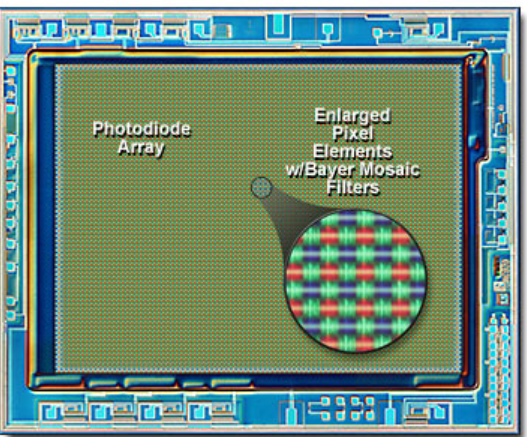
\includegraphics[width=0.4\linewidth]{CCD.png}
	\caption{Schéma d'une CCD : il s'agit d'un tableau de photodiodes (formant les pixels). Ici, on a placé des filtres colorés RVB permettant d'imiter les cônes de l'oeil humain. Source : Florida State University.}
\end{figure}

Ces récepteurs sont sensibles à l'énergie transportée par l'onde lumineuse. Cette énergie est proportionnelle au carré de la vibration lumineuse (nous le démontrerons en électromagnétisme). Par ailleurs, ces capteurs ne sont pas sensibles à la période des oscillations, qui est de l'ordre de $10^{-14}$\,s pour une onde visible. Ils mesurent une moyenne de cette énergie lumineuse sur un grand nombre de périodes. On définit ainsi l'intensité lumineuse :
\begin{definition}
	L'intensité d'une onde lumineuse est définie comme la moyenne du carré de la vibration lumineuse sur un grand nombre de périodes :
	\begin{equation}
		I(\vv r) = \langle s(\vv r,t)^2 \rangle
	\end{equation}
\end{definition}
\begin{remark}
	On définit parfois aussi l'éclairement $\mathcal{E}$. Ces grandeurs ne sont pas tout à fait identiques, mais elles sont toutes deux proportionnelles à la moyenne du carré de la vibration lumineuse, seule chose à retenir en MP.
\end{remark}

En pratique, la moyenne est réalisée sur une période $\tau$ qui dépend du capteur utilisé. Des valeurs de temps caractéristiques sont indiquées dans le tableau suivant :
\begin{table}[h]
	\centering \begin{tabular}{ccc}
		\toprule
		Oeil & CCD & Photodiode \\
		\midrule
		0.1\,s & $10^{-4}$\,s &$10^{-8}$\,s \\
		\bottomrule
	\end{tabular}
	\caption{Temps de réponse de différents capteurs lumineux.}
\end{table}



\section{Onde monochromatique}
Nous allons maintenant nous intéresser plus précisément au cas d'une onde monochromatique. La vibration lumineuse est alors une quantité qui oscille dans le temps, à une fréquence $\nu = \frac{\omega}{2\pi}$. 

Dans ce cas, nous pouvons établir qu'en tout point de l'espace, l'onde va s'écrire :
\begin{equation}
	s(\vv{r},t) = s_0(\vv r) \cos(\omega t - \varphi(\vv r))
\end{equation}

\begin{remark}
Dans ce cours, nous utilisons le retard de phase avec un signe $-$. Il s'agit d'une convention et de nombreuses autres références utilisent plutôt l'avance de phase avec un signe $+$. Dans un sujet de concours, soyez attentifs à la convention choisie, et, si elle n'est pas explicitée dans l'énoncé, choisissez une convention et explicitez-la sur votre copie.
\end{remark}

\begin{definition}[Phase]
	Considérons une onde monochromatique. Le champ scalaire $\phi(\vv r,t) = \omega t - \varphi(\vv r)$ est appelé la phase de l'onde lumineuse. Il dépend du temps.
\end{definition}
\begin{definition}[Retard de phase]
	En considérant la même onde monochromatique, le champ scalaire $\varphi(\vv r)$ est appelé le retard de phase de l'onde lumineuse. Son opposé, $-\varphi(\vv r)$, est l'avance de phase de l'onde lumineuse. Si l'onde est bien monochromatique, ce champ est stationnaire (indépendant du temps).
\end{definition}

\subsection{Fronts d'onde et rayons}

Il est possible de définir les fronts d'onde à partir de la vibration lumineuse :
\begin{definition}
On appelle surface d’onde ou front d’onde une surface continue de l’espace sur laquelle la vibration lumineuse est uniforme à tout instant.
Si les surfaces d’onde sont des sphères concentriques, l’onde est dite sphérique ; s’il s’agit de plans parallèles elle est dite plane.
\end{definition}
\begin{proposition}
Une source ponctuelle émet une onde sphérique, qui peut être approximée par une onde plane à grande distance de la source (c'est-à-dire, si la taille du dispositif d'étude est petite par rapport à la distance entre la source et le dispositif).
\end{proposition}


On constate expérimentalement que l'énergie reçue par un capteur est maximale lorsque le capteur est pointé vers la source lumineuse. Ceci laisse supposer que pour une onde sphérique, l'énergie de l'onde se propage radialement, c'est-à-dire en ligne droite depuis la source vers l'extérieur. Pour représenter cette propagation d'énergie lumineuse, nous définissions les rayons lumineux :
\begin{definition}
	Un rayon lumineux est une ligne le long de laquelle l'énergie lumineuse se propage. C’est une modélisation : on ne peut pas produire ni même isoler un seul rayon lumineux, mais seulement des faisceaux composés d’une infinité de rayons lumineux. Une source ponctuelle émet des rayons lumineux dans toutes les directions. 
\end{definition}
\begin{remark}
	En fin d'année, nous définirons le vecteur de Poynting $\vv \Pi(\vv r,t)$, qui indique la densité volumique de flux énergétique électromagnétique. Les rayons lumineux sont les lignes de champ du vecteur de Poynting, c'est-à-dire qu'elles sont en tout point tangentes à ce champ.
\end{remark}

Pour une onde sphérique, nous venons de voir que l'expérience montre que les rayons lumieux sont radiaux (orientés selon $\vv{e_r}$). Ils sont ainsi perpendiculaires aux surfaces d'onde, d'équation $r = c^{ste}$. Cette propriété se généralise à toutes les ondes lumineuses monochromatiques :
\begin{theorem}[Théorème de Malus (admis)]
Les fronts d'ondes et les rayons d'une onde lumineuse monochromatique sont perpendiculaires en tout point de l'espace.
\end{theorem}

Ce théorème est très important car il permet de faire le lien entre l'aspect ondulatoire de la lumière et l'optique géométrique. Pour mieux le comprendre, on rappelle la définition de deux points conjugués par un système optique :
\begin{definition}[Stigmatisme et conjgaison (révisions)]
Un système optique est dit stigmatique lorsque tous les rayons issus d'un point $A$ et ayant traversé le système optique passent par un point $A'$. $A'$ est alors l'image de $A$ par le système optique et on dit que les points $A$ et $A'$ sont conjugués. Si le prolongement des rayons émergents passe par $A'$, on dit que $A'$ est une image virtuelle de $A$.
\end{definition}
A partir de cette définition, on peut alors représenter l'effet de divers instruments d'optique sur les surfaces et fronts d'onde.

Par exemple, on peut considérer une lentille convergente, qui fait d'un objet réel $AB$ une image réelle $A'B'$. Le théorème de Malus nous permet directement de représenter les surfaces d'onde qui sont perpendiculaires aux rayons :

\begin{figure}[htbp]
    \centering
    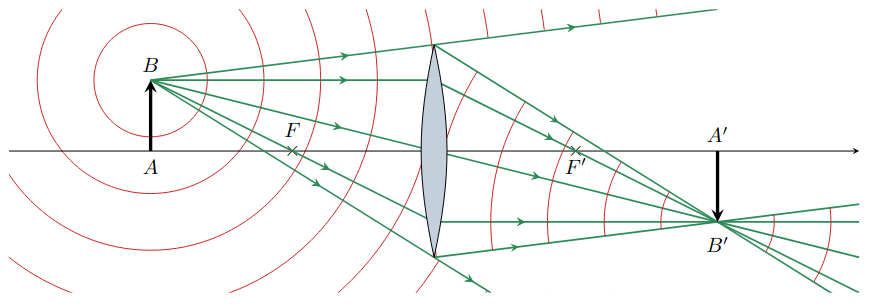
\includegraphics[width=\linewidth]{image_lentille.png}
    \caption{Effet d'une lentille sur les surfaces d'onde. Source : poly de cours de Etienne Thibierge.}
\label{fig:lentille}
\end{figure}

\begin{remark}
D'autres d'exemples de ce type avec des lentilles minces seront traités en TD.
\end{remark}

\begin{capex}
	Représenter l'action d'un miroir plan sur les rayons et les sufaces d'onde d'une onde plane en incidence oblique. Faire de même pour une onde sphérique. En déduire l'interprétation de la formation d'une image en termes de surface d'onde.
\end{capex}





\section{Chemin optique}

\subsection{Onde plane monochromatique, vecteur d'onde}

Nous allons maintenant nous intéresser plus particulièrement à une onde plane afin de mieux comprendre sa structure. La vitesse de propagation de l'once est $c_{onde} = \frac{c}{n}$ où $c$ est la vitesse de la lumière dans le vide, et $n$ l'indice optique du milieu. Si l'on suppose que l'onde se propage dans la direction $+\vv{e_x}$, on s'attend à ce qu'elle soit de la forme :
 \begin{equation}
	 s = f(x - c_{onde}t) = g \left(t-\frac{n x}{c}\right)
\end{equation}
(L'éventuel terme en $f'(x + c_{onde}t)$ n'est pas à considérer ici puisqu'il correspond à une propagation en sens opposé, selon $- \vv{e_x}$).

En comparant cette expression à l'expression de la phase, nous obtenons la relation suivante :
\begin{equation}
\varphi(\vv r,t) = \omega \frac{n x}{c} + \varphi_0
\end{equation}
où $\varphi_0$ est une constante. On pourra alors écrire :
\begin{equation}
	s(x,t) = s_0 \cos(\omega t - k_x x - \varphi_0)  
\end{equation}
où $k_x = \frac{\omega n}{c}$.
Cette onde a une périodicité spatiale $\lambda = \frac{2\pi}{k}$ dans la direction $x$. Cette propriété se généralise en trois dimensions, et permet d'étudier la propagation d'une onde plane de direction quelconque.

\begin{definition}
On définit le vecteur d'onde $\vv k$ tel qu'une onde lumineuse plane monochromatique s'écrive de la forme :
\begin{equation}
	s(\vv r,t) = s_0 \cos(\omega t - \vv k \cdot \vv r + \varphi_0)
\end{equation}
Le vecteur d'onde est alors relié à la longueur d'onde par la relation :
\begin{equation}
	\lambda = \frac{2\pi}{||\vv k||}
\end{equation}
Et les rayons lumineux sont orientés dans la direction du vecteur $\vv k$.
\end{definition}

\subsection{Onde sphérique monochromatique}

Dans le cas d'une onde sphérique, nous avons pu montrer expérimentalement que l'intensité lumineuse associée à l'onde, $\langle s^2 \rangle$ décroît comme le carré de la distance $r$. Ceci nous permet d'établir la forme de l'onde sphérique :
\begin{proposition}[Forme d'une onde sphérique (admise)]
Une onde sphérique monochromatique peur s'écrire sous la forme :
\begin{equation}
	s(r,t) = \frac{s_0}{r} \cos\left(\omega\left(t-\frac{n r}{c}\right) - \varphi_0\right)
\end{equation}
\end{proposition}
On constate qu'à l'intérieur du cosinus, la phase de l'onde $\phi$ a exactement la même expression que la phase d'une onde plane, pour peu que l'on remplace la coordonnée linéaire $x$ par le rayon $r$.

\subsection{Chemin optique}

L'analyse de l'onde sphérique comme de l'onde plane nous montre que la forme générale de la phase de l'onde $\phi$ ne dépend pas de la nature de l'onde (plane ou sphérique). Pour exprimer cette phase, nous définisssons le chemin optique :
\begin{definition}
	Le chemin optique entre deux points $A$ et $B$, calculé le long d'un rayon lumineux, est donné par :
	\begin{equation}
		(AB) = \int_A^B n \dd \ell
	\end{equation}
	où $\dd \ell$ est la distance élémentaire le long du rayon lumineux considéré. Le chemin optique dépend du chemin suivi, il est donc important de préciser le long de quel rayon il est calculé.
\end{definition}
\begin{remark}
	Dans un milieu homogène, le chemin optique est simplement le produit de la distance géométrique par l’indice optique. Pour un rayon en ligne droite, on a ainsi $(AB) = n AB$.
\end{remark}

\begin{capex}
	Déterminer la phase d'une onde monochromatique issue d'une source $S$ en un point de l'espace $A$ en fonction du chemin optique $(SA)$ parcouru le long d'un rayon. En déduire la propriété suivante.
\end{capex}
\begin{proposition}
Le déphasage d’une onde entre deux points $M$ et $M'$ se trouvant sur un même rayon lumineux est relié au chemin optique entre ces deux points :
	\begin{equation}
	\varphi(M') - \varphi(M) = \frac{2\pi}{\lambda} (MM')
	\end{equation}
\end{proposition}


\begin{encart}[Mesures des séismes par InSAR]
	Cette propriété est directement utilisée par la méthode InSAR, développée en 2006, et qui permet de visualiser des mouvements de terrain lors d'un séisme ou d'une éruption volcanique. Le principe est simple : un satellite en orbite basse (altitude de quelques centaines de kilomètres) envoie une onde électromagnétique vers le sol. L'onde est réfléchie par le sol et renvoyée vers le satellite, qui mesure le signal obtenu. On peut alors mesurer le déphasage entre l'onde envoyée et l'onde reçue, autrement dit, on mesure à une constante près la phase $\Phi$ de l'onde.

	Lorsqu'un séisme se produit, on peut calculer la différence de phase entre la phase mesurée avant et après le séisme. La relation que nous venons de démontrer implique que :
	\begin{equation}
		\Delta r = \frac{\delta}{2} = \frac{\Delta \varphi}{4\pi}\lambda
	\end{equation}
	où $\delta$ est la différence de marche entre les deux rayons aller-retour, qui correspond au double de la variation de hauteur du sol dans la direction de visée, $\Delta r$. La longueur d'onde est choisie dans le domaine radar ($\lambda \sim 10$\,cm), ce qui permet de mesurer des déplacements centimétriques. Le principe est détaillé sur la figure suivante.

	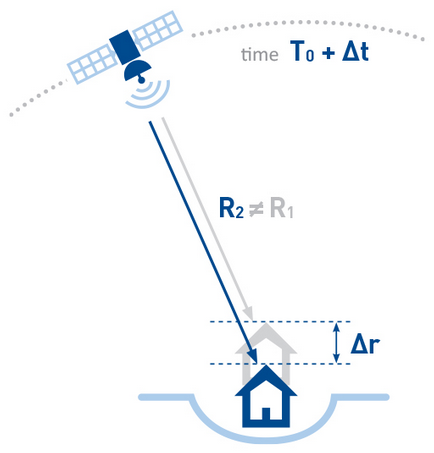
\includegraphics[width=0.35\linewidth]{principe_SAR.png} 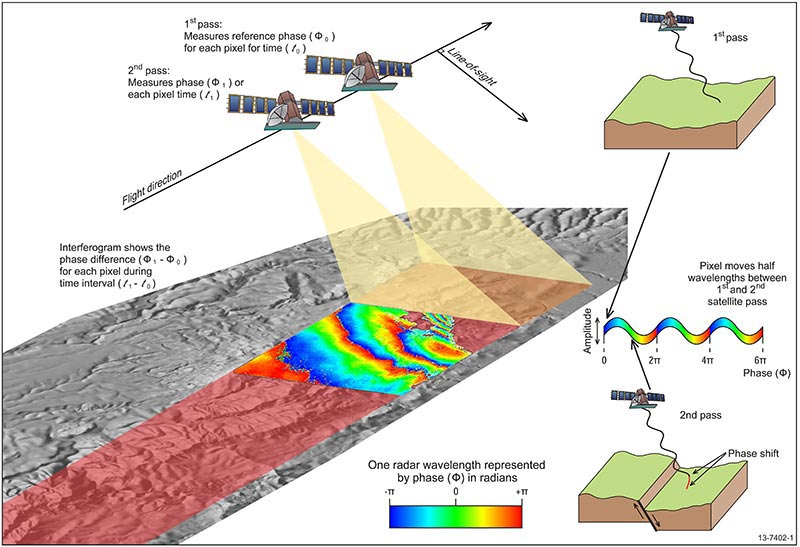
\includegraphics[width=0.6\linewidth]{principe_insar.jpg}


	Les images ci-dessous montrent des mesures réalisées par InSAR montrant le gonflement du volcan South Sister dans l'Oregon aux Etats-Unis, ainsi qu'une estimation du déplacement du sol lors du séisme qui a frappé Haïti en 2010 (image réalisée par un groupe de charcheurs et chercheuses américains et haïtiens).
\end{encart}



\begin{figure}[p]
    \centering
    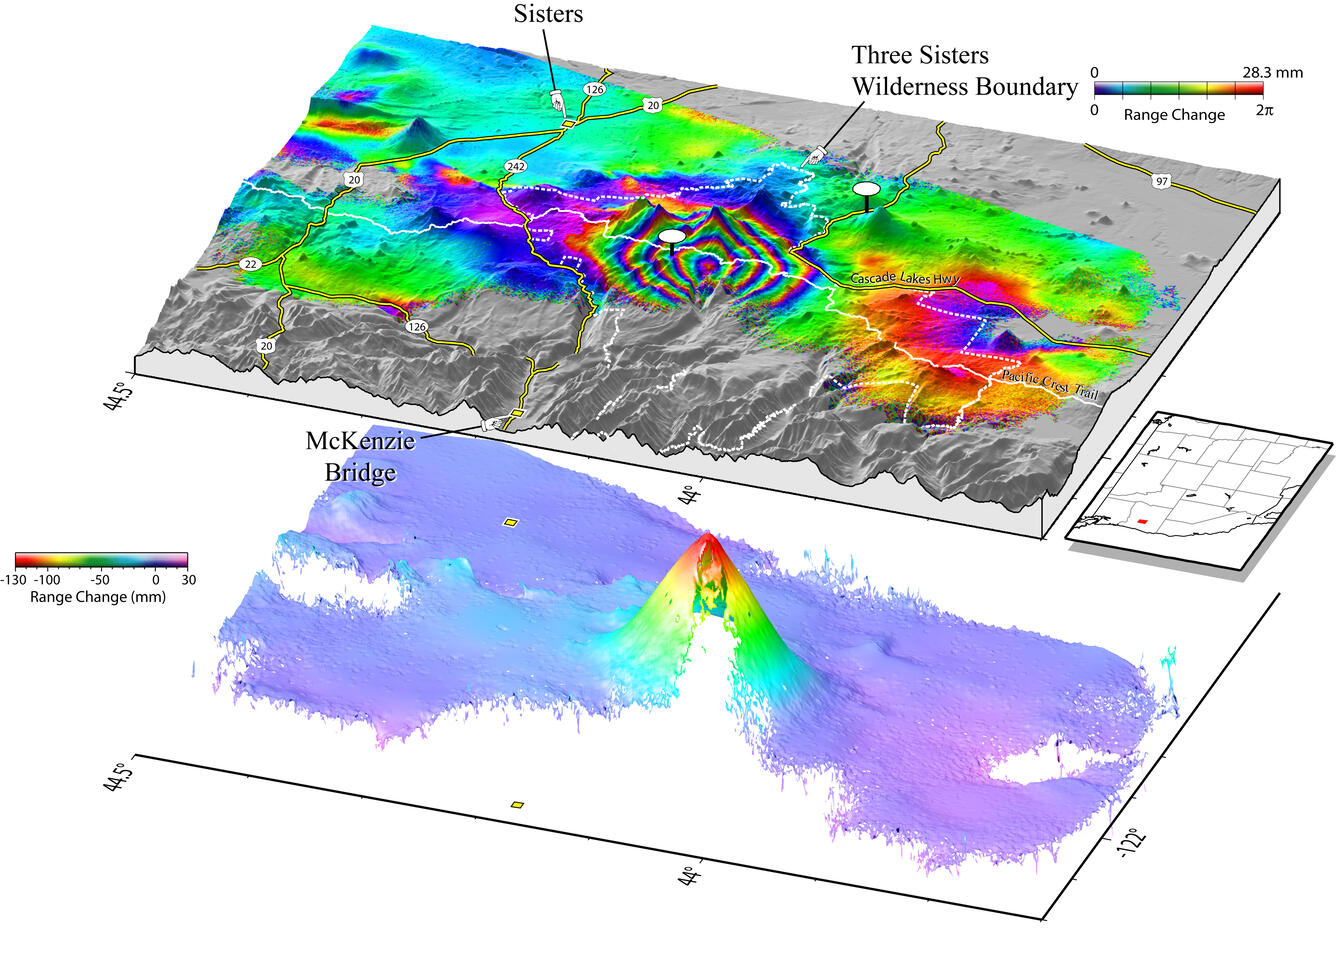
\includegraphics[width=\linewidth]{insar_volcan.jpg}
    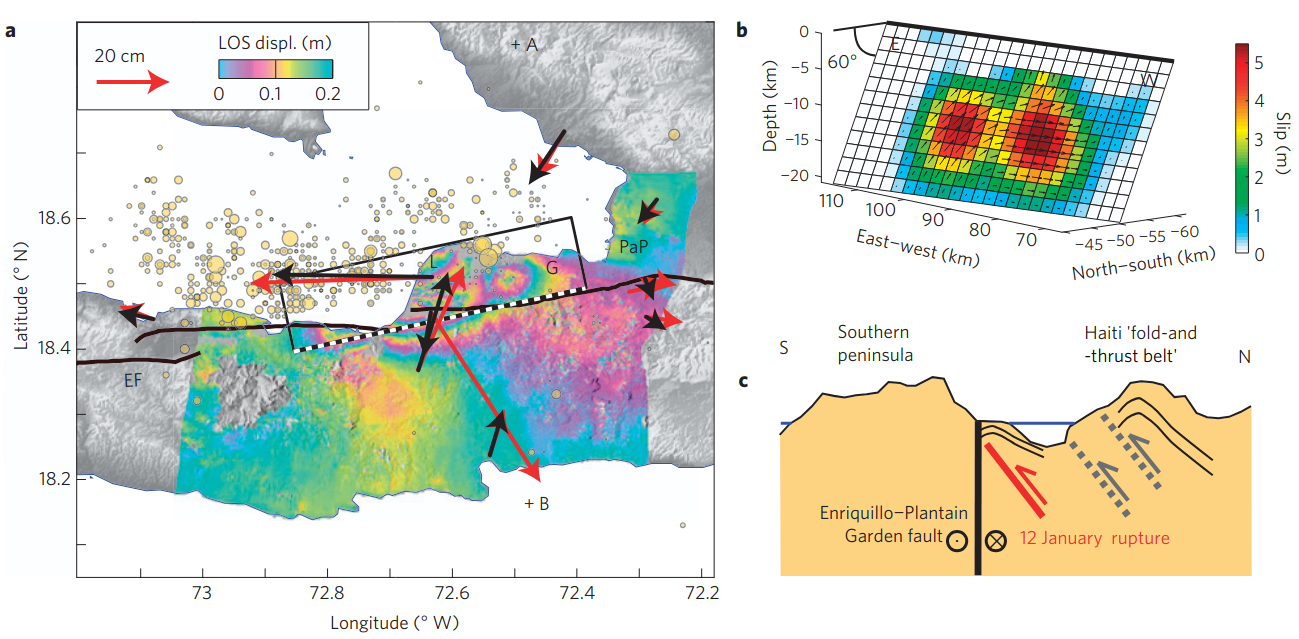
\includegraphics[width=\linewidth]{papier_haiti.png}
	\caption{En haut : déformation du volcan South Sister aux Etats Unis. Source : USGS (United States Geological Survey). En bas : mesure de la différence de phase cau sée par le séisme de Haïti en 2010 (a) et estimation du mouvement total le long de la faille (b). Source : Calais et al. (2010). \textit{Transpressional rupture of an unmapped fault during the 2010 Haiti earthquake.} Nature Geoscience, 3(11), 794-799.}
\end{figure}



\begin{capex}
Que peut-on dire du chemin optique entre une source lumineuse et deux points d'une même surface d'onde ? En déduire la propriété suivante.
\end{capex}

\begin{proposition}[Chemin optique entre points conjugués]
	Le chemin optique séparant deux points conjugués par un système optique est indépendant du rayon lumineux choisi.
\end{proposition}

Cette propriété est bien visible, par exemple, sur la figure \ref{fig:lentille} : les rayons pour lesquels la distance géométrique est la plus courte ont un parcours plus long dans le verre de la lentille. Comme le verre a un indice optique $n>1$, ceci contribue à augmenter le chemin optique total, et donc à compenser la longueur plus courte du trajet lumineux.



\subsection{Principe de superposition}

Les équations de l'électromagnétisme (que nous n'avons pas encore vues), sont des équations linéaires. Nous pouvons en déduire que le principe de superposition s'applique non pas à l'intensité lumineuse $I$, mais à la vibration lumineuse $s$ :
\begin{theorem}[Principe de superposition]
	Soient $s_1$ et $s_2$ deux ondes lumineuses créées par les sources respectives $S_1$ et $S_2$. Alors l'onde créée par l'ensemble des deux sources $S_1 \cup S_2$ est $s_1+s_2$.
\end{theorem}
\label{fresnel_v1}

\begin{capex}
Etablir l'intensité résultant de la superposition de deux ondes monochromatiques de fréquence $\nu_1$ et $\nu_2$ en un point $M$ de l'espace. Mettre en évidence l'existence d'un termes d'interférences.
\end{capex}

On constate que les intensités lumineuses, à la différence de la vibration lumineuse, ne satisfont pas forcément le principe de superposition. Ceci nous permet de définir la notion d'interférences lumineuses :
\begin{definition}
	On dit qu’il y a interférences entre deux ondes lorsque l’intensité issue de la superposition de ces deux ondes n’est pas égale à la somme des intensités de chaque onde individuelle. Deux ondes pouvant interférer sont dites cohérentes.
\end{definition}

La formule obtenue nous amène à distanguer deux cas, dans lesquels on dira que les ondes lumineuses sont soit cohérentes, soit incohérentes. Dans le cas où les ondes sont cohérentes, le terme d'interférences sera non nul. Pour cela, nous avons besoin de revenir plus en détail sur l'émission et la mesure de la lumière.


\section{Notion de cohérence}

Nous souhaitons comprendre si deux ondes seront cohérentes, c'est-à-dire si le terme d'interférences pourra avoir une moyenne non nulle :
\begin{equation}
	\langle \cos \left( 2 \pi (\nu_1 - \nu_2) t + \varphi_1(\vv r) - \varphi_2(\vv r) \right) \rangle \neq 0
\end{equation}

Pour cela, il y a deux conditions de cohérence pour les vibrations lumineuses :
\begin{itemize}
	\item Les ondes ont la même fréquence centrale ($\nu_1 = \nu_2$)
	\item Leur déphasage varie lentement par rapport aux temps caractéristiques de l'expérience ($\varphi_1(\vv r) - \varphi_2(\vv r)$ reste constant)
\end{itemize}

Pour pouvoir interpréter ces conditions de manière plus concrète, il est nécessaire de décrire de manière un peu plus précise les propriétés des ondes.

\subsection{Modèle d'émission des ondes lumineuses. Temps de cohérence.}

En pratique, le spectre d’une onde lumineuse ne peut jamais être parfaitement pur, pas même celui d’un laser ou si l’on isole une raie à l’aide d’un filtre coloré. Ainsi, une onde lumineuse n’est jamais parfaitement sinusoïdale, c’est-à-dire que les paramètres de la sinusoïde (amplitude, fréquence, phase initiale) varient lentement au cours du temps. Logiquement, le temps caractéristique de ces variations lentes doit se retrouver sur le spectre.

\begin{definition}
	On appelle temps de cohérence $\tau_c$ d’une source lumineuse le temps caractéristique de variation des propriétés de l’onde lumineuse. On définit également la longueur de cohérence $\ell_c = c \tau_c$, qui correspond à la distance parcourue par l'onde pendant le temps de cohérence.
\end{definition}

Le temps de cohérence d'une onde lumineuse peut être relié au spectre d'émission de la source $I_\nu(\nu)$, qui indique l'intensité lumineuse de la source en fonction de la fréquence :
\begin{equation}
	I = \int_0^\infty I_\nu(\nu) \dd \nu
\end{equation}

\begin{remark}
	Le théorème de Parseval (hors programme) permet de décomposer l'intensité d'une onde lumineuse, égale à la moyenne de son carré, en un spectre énergétique :
	\begin{equation}
		\int_{-\infty}^\infty |\underline{s}(t)|^2 \dd t = \int_0^\infty |\hat{s}(\nu)|^2 \dd \nu
	\end{equation}
	où $\hat{s}(\nu)$ est la transformée de Fourier continue du signal :
	\begin{equation}
		\hat{s}(\nu) = \int_{-\infty}^\infty s(t) e^{-j 2 \pi \nu t} \dd t
	\end{equation}
	Autrement dit, l'intensité lumineuse peut se décomposer comme une intégrale sur la fréquence, et on appellera $I_\nu(\nu) = |\hat{s}(\nu)|^2$ le spectre d'émission d'une source lumineuse.
\end{remark}

\begin{example}
\textit{La connaissance de cet exemple n'est pas exigible, mais est vivement recommandée aux personnes qui envisagent de passer les concours les plus difficiles (Mines/Centrale/X/ENS).}
Considérons une onde sinusoïdale amortie dans le temps :
	\begin{equation}
		s(t) = s_0 e^{-t/\tau_c} \cos(2 \pi \nu_0 t)
	\end{equation}
	qui se modélise par l'onde complexe :
	\begin{equation}
		\underline{s}(t) = s_0 e^{j 2 \pi \nu_0 t - t/\tau_c}
	\end{equation}
$\tau_c$ est alors le temps de cohérence de cette onde (en l'occurence, ici, c'est le temps caractéristique de variation de son amplitude).
Quel est le spectre de cette onde ? Pour le savoir, nous pouvons en faire la transformée de Fourier :
	\begin{align}
		\hat{s}(\nu) &= \int_0^\infty s(t) e^{-j 2 \pi \nu t} \dd t  \\
		&= s_0 \int_0^\infty  \exp\left( \left(j 2 \pi(\nu_0-\nu)-\frac{1}{\tau_c}\right)t \right)  \\
		&= \frac{s_0}{\frac{1}{\tau_c} + 2 \pi j(\nu-\nu_0)}
	\end{align}
On obtient ainsi l'expression du spectre :
	\begin{equation}
		I_\nu(\nu) = \frac{s_0^2 \tau_c^2}{1 + 4 \pi^2 \tau_c^2 (\nu-\nu_0)^2}
	\end{equation}
On constate que la largeur spectrale de la courbe à mi-hauteur est telle que $4 \pi^2 \tau_c^2 (\Delta \nu / 2)^2 = 1$ soit :
\begin{equation}
	\Delta \nu \times \tau_c = \frac{1}{\pi}
\end{equation} 
\end{example}

De manière générale, on admettra et on retiendra la propriété suivante :
\begin{proposition}
	La largeur spectrale d'une source, $\Delta \nu$, est reliée à son temps de cohérence $\tau_c$ par la relation :
	\begin{equation}
		\Delta \nu \times \tau_c \approx 1
	\end{equation}	
\end{proposition}

\begin{capex}
	Utiliser cette relation pour déterminer le lien entre le temps de cohérence et la largeur spectrale de la source, évaluée en termes d'incertitude sur la longueur d'onde émise $\Delta \lambda$.
\end{capex}

\paragraph{Le modèle des trains d'onde}

A priori, l’onde lumineuse est une onde presque harmonique, dont l’amplitude, la fréquence et la phase initiale peuvent varier de manière simultanée : de telles variations combinées ne peuvent pas être décrites mathématiquement de façon simple. Le modèle des trains d’onde est une simplification permettant de décrire efficacement une onde lumineuse. Il inclut l'effet de temps de cohérence en restant relativement simple.

\begin{definition}[Modèle des trains d'onde]
	Une onde lumineuse est modélisée par une succession de trains d’onde, tous de même durée $\tau_c$, pendant lesquels l’onde est parfaitement sinusoïdale. Entre deux trains d’onde, la phase subit une discontinuité aléatoire, alors que l’amplitude et la fréquence restent inchangées.
\end{definition}


\begin{figure}[htbp]
    \centering
	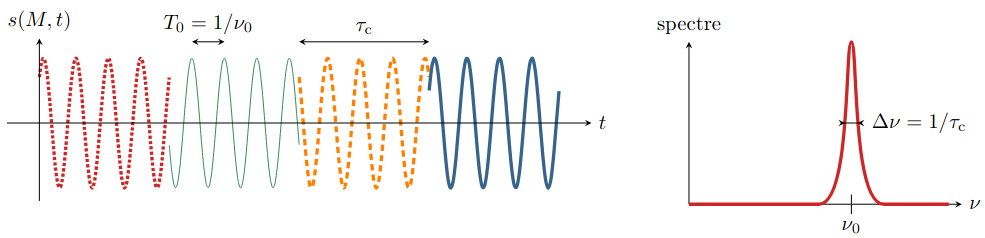
\includegraphics[width=\linewidth]{trains_onde.png}
	\caption{Le modèle du train d'ondes. Source : poly de cours de Etienne Thibierge.}
\end{figure}

On a alors la propriété suivante :
\begin{proposition}[Longueur d'un train d'onde]
La longueur des trains d'onde correspond à la longueur de cohérence $\ell_c$ de la source lumineuse.
\end{proposition}

\paragraph{Quelques sources lumineuses}

Nous allons maintenant nous intéresser à quelques sources lumineuses.

Les sources thermiques (comme une ampoule à incandescence) émettent un spectre donné qui satisfait la loi de Wien, vue au lycée. Il s'agit d'un spectre très large, dont la largeur est du même ordre de grandeur que la longueur d'onde centrale. On a ainsi $\Delta \nu \sim \nu_0$, ce qui implique que le temps de cohérence est du même ordre de grandeur que la péruiode de l'onde : $\tau_c \sim 10^{-14}$\,s. La longueur de cohérence est de l'ordre d'une longueur d'onde ($10^{-6}$\,m)

Les lampes à vapeur, en revanche, émettent une lumière avec un spectre très piqué, si bien que leur longueur de cohérence est nettement plus importante. Pour une lampe à vapeur de mercure classique, on aura $\lambda = 546.07$\,nm et $\Delta \lambda = 0.02$\,nm. Ceci implique un temps de cohérence :
\begin{equation}
	\tau_c = \frac{1}{\Delta \nu} = \frac{\lambda^2}{c \Delta \lambda} \sim 10^{-10}\,\mathrm{s}
\end{equation}

Enfin, le laser présente un temps de cohérence encore plus long que les sources spectrales.

Voici quelques ordres de grandeurs de temps et de longueurs de cohérence pour différents trains d'onde :
\begin{table}[h]
	\centering \begin{tabular}{cccc}
		\toprule
		&Lumière blanche & Raie spectrale & Laser \\
		\midrule
		$\tau_c$\,[s] & $10^{-14}$ & $10^{-10}$ & $10^{-8}$ \\
		$\ell_c$\,[m] & $10^{-6}$ & $10^{-2}$ & $1$ \\
		\bottomrule
	\end{tabular}
	\caption{Temps et longueur de cohérence de différentes sources lumineuses.}
\end{table}

\subsubsection{Interférences, trains d'onde et longueur de cohérence}

Nous pouvons désormais revenir sur notre seconde condition pour que les ondes soient cohérentes : il faut que $\varphi_1(M,t) - \varphi_2(M,t)$ soit constant. Sachant que le déphasage entre deux trains d'onde différent est aléatoire, il faut que les deux vibrations lumineuses au point $M$ appartiennent au \textbf{même train d'onde} :
\begin{proposition}
	Pour que deux vibrations lumineuses soient cohérentes, elles doivent appartenir au même train d'onde.
\end{proposition}

Cela est évidemment impossible pour des sources physiquement différentes. Ainsi, pour faire interférer deux ondes, il est nécessaire de crééer deux sources secondaires à partir d'une source primaire. Pour cela, nous verrons deux types de dispositifs : les dispositifs à division d'amplitude et les dispositifs à division de front d'onde. Dans les deux cas, les deux ondes $s_1$ et $s_2$ sont issues de la même source primaire, mais n'ont pas parcouru les mêmes rayons lumineux. Elles ont donc un chemin optique différent, ce qui induit un déphasage.

On définit alors la différence de marche des deux rayons :
\begin{definition}[Différence de marche]
	La différence de marche entre deux ondes lumineuses $s_1$ et $s_2$ atteignant un même point $M$ est donnée par la différence de chemin optique entre ces deux rayons (notés 1 et 2) depuis une même source primaire $S$ :
	\begin{equation}
		\delta = (SM)_2 - (SM)_1
	\end{equation}
\end{definition}

\begin{capex}
Traduire la condition de cohérence sur les trains d'onde en une inégalité sur la longueur de cohérence de la source primaire et la différence de marche entre les deux rayons parcourus par chacune des ondes.
\end{capex}

On aboutit aux conditions de cohérence suivantes :
\begin{proposition}[Cohérence de deux ondes]
Deux ondes sont cohérentes en un point $M$ de l'espace, si et seulement si :
\begin{itemize}
	\item Elles ont même longueur d'onde ;
	\item Elles proviennent d'une même source primaire ;
	\item La différence de marche $\delta$ entre les deux ondes au point $M$ est inférieure à la longueur de cohérence de l'onde : $\delta < \ell_c$. 
\end{itemize}
\end{proposition}
\begin{remark}
	On peut remarquer que la première condition est automatiquement vérifiée si la seconde l'est. On pourrait donc la retirer de la liste, mais il est bon de se rappeler de cette condition séparément car les conditions 1 et 2 viennent de l'analyse de termes séparés dans l'équation.
\end{remark}

\section{Interférences à deux ondes}

\subsection{Formule de Fresnel}

Nous pouvons maintenant utiliser la notion de cohérence pour étudier de manière théorique les interférences à deux ondes.
\begin{capex}
En réutilisant le résultat établi en section \ref{fresnel_v1}, appliqué au cas de deux ondes cohérentes, déterminer l'intensité de chacune des deux ondes en fonction de leur intensités respectives et de leur déphasage.
\end{capex}
Nous obtenons la formule de Fresnel :
\begin{theorem}[Formule de Fresnel]
	Soient deux ondes $s_1$ et $s_2$ se superposant en un point $M$. Si ces ondes sont cohérentes, alors l'intensité de la superposition des ondes s'écrit :
	\begin{equation}
		I_{tot} = I_1 + I_2 + \sqrt{I_1 I_2} \cos(\varphi_1(M) - \varphi_2(M))
	\end{equation}
\end{theorem}

Notons que nous pouvons réécrire cette formule en termes de différence de marche, en remarquant que le déphasage s'écrit $\Delta \varphi = 2 \pi \frac{\delta}{\lambda}$ :

\begin{proposition}
	Soient deux ondes $s_1$ et $s_2$ se superposant en un point $M$. Si ces ondes sont issues d'une même source primaire et ont une différence de marche $\delta < \ell_c$ où $\ell_c$ est la longueur de cohérence de la source, alors :
	\begin{equation}
		I_{tot}(M) = I_1 + I_2 + \sqrt{I_1 I_2} \cos(2 \pi \delta(M))
	\end{equation}
\end{proposition}

\subsection{Interférences constructives et desctructives}

On constate que la superposition de deux ondes monochromatiques d'intensité uniforme a une intensité non uniforme. En effet, $I_{tot}$ dépend de la position $M$ alors que ce n'est le cas ni de $I_1$, ni de $I_2$.

\begin{definition}
Une \textbf{figure d'interférences} correspond au motif dessiné par des variations d'intensité lumineuse dans l'espace lorsqu'on a une superposition de deux ondes cohérentes.

On appelle \textbf{champ d'interférences} la région de l'espace dans laquelle les deux ondes se superpose, où on peut observer la figure d'interférences.

Dans les zones où l'intensité est plus faible que la moyenne, le termes d'interférences est négatif et on dit que les interférences sont \textbf{desctructives}.

Au contraire, dans les zones où l'intensité est plus élevée que la moyenne, le terme d'interférences est positif et on dit que les interférences sont \textbf{constructives}.
\end{definition}

\begin{example}[Interférence de deux ondes sphériques]
	Supposons que l'on a deux ondes sphériques issues de deux sources secondaires cohérentes. Un tel dispositif peut être construit, par exemple, à partir des miroirs de Fresnel : 	On suppose les deux sources placées sur l'axe $(Oy)$. Nous souhaitons étudier l'allure de la figure d'interférences sur deux écrans représentés sur la figure suivante. Nous allons étudier les propriétés de symétrie de la situation pour en déduire l'allure de la figure d'interférences.
\begin{itemize}
	\item Sur l'écran 1 : si l'on est suffisamment proche du plan $(xOy)$, la différence de marche est essentiellement due à la différence de chemin optique à parcourir le long de l'axe $(Oy)$, elle est donc invariante par translation selon $\vv{e_z}$. Ainsi, l'intensité est également invariante par translation delon $\vv{e_z}$ et on va observer des franges.
	\item Sur l'écran 2 : la différence de marche est invariante par rotation autour de $(Oz)$, il en est donc de même pour l'intensité lumineuse : la figure d'interférences correspond à des anneaux centrés sur l'axe $(Oz)$.
\end{itemize}
\end{example}


\begin{figure}[htbp]
    \centering
	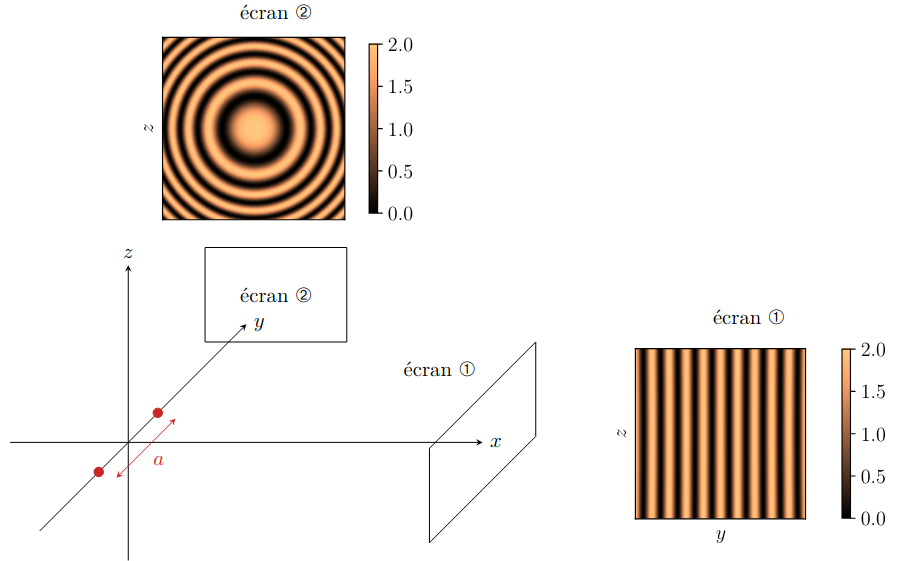
\includegraphics[width=\linewidth]{interferences_deux_ondes.png}
	\caption{Interférence de deux ondes issues de deux sources ponctuelles secondaires. Source : poly de cours de Etienne Thibierge.}
\end{figure}


\begin{figure}[t]
	\centering
	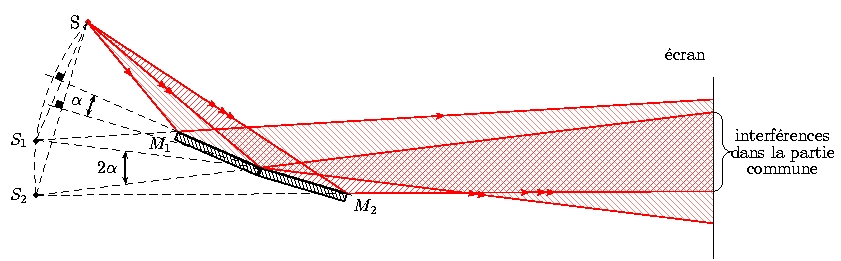
\includegraphics[width=\linewidth]{fresnel_mirror.jpg} 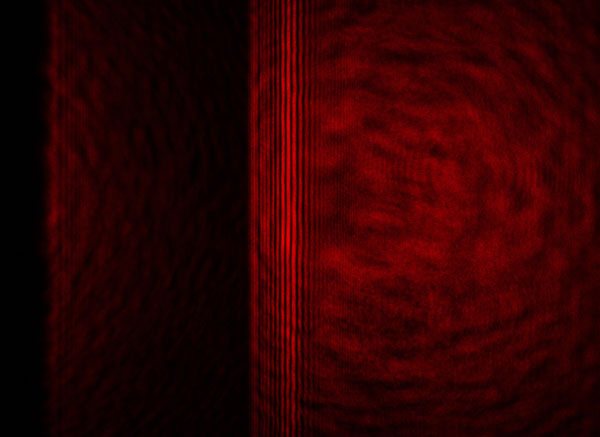
\includegraphics[width=0.65\linewidth]{fresnel_photo.jpg}
	\caption{Les miroirs de Fresnel. En haut : schéma du dispositif. En bas : photo des interférences observées. Sources : melusine.eu.org et Leybold.}
\end{figure}



\begin{encart}[Les miroirs de Fresnel]
	Une des premières expériences à avoir démontré le caractère ondulatoire de la lumière est celle des miroirs de Fresnel : on fait l'image d'une source primaire $S$ par deux miroirs légèrement inclinés, ce qui crée deux sources virtuelles secondaires $S_1$ et $S_2$, comme indiqué sur la figure ci-dessous.
	On se retrouve alors dans la situation précédente, et en pratique on observe les franges lumineuses. Dans son compte rendu d'expérience, Fresnel fait les observations suivantes :
	\begin{displayquote}
	{\small Nous pouvons maintenant expliquer celle des deux miroirs, dans laquelle on obtient des effets très frappants de l'influence mutuelle des rayons lumineux par la réunion de deux faisceaux réfléchis régulièrement sur leur surface. Il ne faut point employer de glaces étamées, mais noircies par derrière, afin de détruire la seconde réflexion, qui compliquerait le phénomène ; des miroirs métalliques sont encore préférables. Après avoir placé les deux miroirs l'un à côté de l'autre, et de sorte que leurs bords se touchent parfaitement, on les fait tourner jusqu'à ce qu'ils se trouvent presque dans le même plan, et forment néanmoins entre eux un angle légèrement rentrant, de manière à présenter à la fois deux images du point lumineux. On peut juger de cet angle d'après l'intervalle qui sépare les images ; il faut que cet intervalle soit petit pour que les franges aient une largeur suffisante. Mais une chose à laquelle on doit apporter le plus grand soin, c'est que les miroirs ne saillent pas l'un sur l'autre dans la ligne de contact, car une saillie d'un ou deux centièmes de millimètre suffirait souvent pour empêcher l'apparition des franges. On parvient à remplir cette condition par le tâtonnement, en pressant peu à peu celui des deux miroirs que l'on croit le plus saillant contre la cire molle au moyen de laquelle on les a fixés sur un appui commun ; et l'on juge au tact, et mieux encore en cherchant les franges à l'aide de la loupe, si la condition est remplie. On pourrait sans doute imaginer un mécanisme au moyen duquel on ferait varier à volonté l'angle des deux miroirs, en évitant toute saillie de l'un sur l'autre ; mais il faudrait qu'il fût construit avec un grand soin. Si le procédé que je viens d'indiquer est plus long par les tâtonnements qu'il nécessite, il a dit moins l'avantage de n'exiger d'autre appareil que deux petits miroirs de métal ou verre noir, et d'être ainsi à la portée de tout le monde.

On ne doit employer dans cette expérience, comme dans celles de diffraction, que la lumière d'un seul point lumineux [...]

Alors on cherche les franges dans l'espace où se réunissent les rayons réfléchis sur les deux miroirs, qu'il est facile de distinguer du reste du champ lumineux à la supériorité de son éclat.

Ces franges présentent une série de bandes brillantes et obscures, parallèles entre elles, et à égales distances les unes des autres. Dans la lumière blanche elles sont parées des plus vives couleurs, surtout celles qui avoisinent le centre ; car, à mesure qu'elles s'en éloignent, elles s'affaiblissent graduellement, et disparaissent enfin vers le huitième ordre. Dans une lumière plus homogène, telle que celle qu'on peut obtenir au moyen d'un prisme ou de certains verres colorés en rouge on aperçoit un bien plus grand nombre de franges, qui ne présentent plus alors qu'une suite de bandes obscures et brillantes de même couleur.

La direction de ces bandes est toujours perpendiculaire à la ligne droite qui joindrait les deux images du point lumineux, du moins dans l'espace éclairé par la lumière régulièrement réfléchie, quelle que soit la direction de cette ligne relativement aux bords des miroirs en contact ; ce qui prouve bien qu'elles né proviennent pas d'une influence exercée par ces bords sur les rayons lumineux qui passent dans leur voisinage. On peut d'ailleurs, en augmentant l'angle des miroirs, écarter assez l'une de l'autre les deux images du point lumineux, pour que les rayons qui concourent à la production des franges soient réfléchis à des distances telles des bords en contact, qu'on ne puisse plus supposer aucune action sensible, de leur part.

La bande centrale est brillante, comme dans tes franges qui divisent l'ombre d'un corps étroit, ou celles qu'on obtient au moyen d'un écran percé de deux fentes parallèles, et suffisamment rapprochées. Cette bande brillante est placée entre deux bandes obscures du noir le plus foncé, quand un emploie, comme nous le supposons, une lumière sensiblement homogène ; chacune d'elles est suivie d'une bande brillante à laquelle succède de nouveau une bande obscure et ainsi suite. Les bandes obscures sont encore d'un noir très foncé dans les franges du deuxième et du troisième ordre ; mais, à mesure qu'on s'éloigne du centre, elles deviennent moins prononcées, ce qui tient à ce que la lumière employée n'est jamais parfaitement homogène.

Il suffit, de comparer les bandes obscures des premier, deuxième et troisième ordres à la lumière donnée par un seul miroir, pour se convaincre qu'elles sont beaucoup, moins éclairées, et que, dans les positions qu'elles occupent, l'addition des rayons d'un des miroirs à ceux de l'autre, au lieu de former une lumière plus intense, produit de l'obscurité.}
	\end{displayquote}
\end{encart}

\begin{capex}
	A partir des notions de cohérence que nous avons vues, expliquer pourquoi Fresnel observe seulement 8 franges en lumière blanche, et beaucoup plus en lumière monochromatique.
\end{capex}

\subsection{Notion de constraste}

Pour caractériser la visibilité des franges d'interférence, on définit la notion de contraste :
\begin{definition}[Contraste d'une figure d'interférences]
	Le constraste de franges d'interférence est défini comme un rapport fonction des intensités maximale $I_{max}$ et minimale $I_{min}$ de la figure :
	\begin{equation}
		\mathcal{C} = \dfrac{I_{max}-I_{min}}{I_{max}+I_{min}}
	\end{equation}
\end{definition}

\begin{remark}
	Le contraste est parfois appelé \textit{visibilité} et noté $\mathcal{V}$. Attention à ne pas confondre une figure d'interférences mal contrastée avec des interférences destructives ! Le contraste est relié, ici, à une différence d'intensité entre les deux ondes.
\end{remark}

Le contraste est directement relié à la visibilité des franges, comme on le voit sur la figure suivante :

\begin{figure}[htbp]
    \centering
	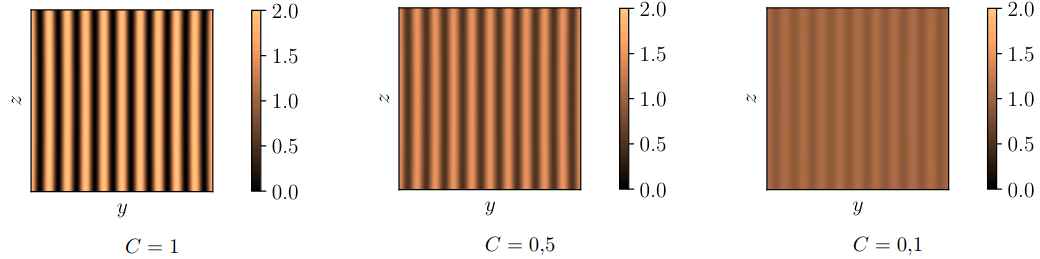
\includegraphics[width=\linewidth]{contraste.png}
	\caption{Franges d'interférences pour différents contrastes. Source : poly de cours de Etienne Thibierge.}
\end{figure}

\begin{capex}
	Exprimer le contraste d'une interférence à deux ondes en fonction des intensités $I_1$ et $I_2$ de chacune des deux ondes. Réécrire la formule de Fresnel en faisant apparaître le contraste $\mathcal{C}$.
\end{capex}
On en déduit la propriété suivante :
\begin{proposition}
	Le contraste d'une figure d'interférence à deux ondes est maximal lorsque les deux ondes ont des intensités voisines.
\end{proposition}

\begin{remark}
	En pratique, nous essayerons toujours de nous placer dans ce type de conditions expérimentalement. Pour les miroirs de Fresnel, ceci revient à éclairer de manière égale chacun des deux miroirs, c'est-à-dire d'avoir un faisceau lumineux bien homogène.
\end{remark}

\begin{figure}[htbp]
	\centering
	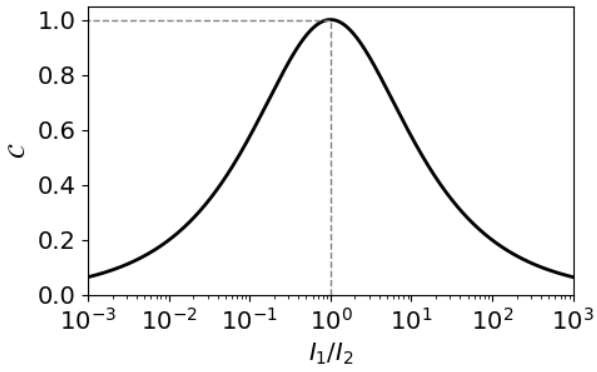
\includegraphics[width=0.5\linewidth]{contraste_fct.png}
	\caption{Contraste de la figure d'interférences en fonction du rapport d'intensité des deux ondes qui interfèrent.}
\end{figure}

\end{document}
